\chapter{Introdução}

Como exposto em \cite{Torralba2008}, o aprendizado de máquina tem sido utilizado como alternativa à implementação de algoritmos específicos e complexos durante a resolução de diversos tipos de problemas. 

\lipsum[6]

A Figura \ref{fig:mlapplications}, apresenta um breve resumo das possíveis aplicações do aprendizado de máquina.

\begin{figure}[ht]
    \centering
    \caption{Domínio de aplicações do aprendizado de máquina.}
    \copyrightbox[b]
    		{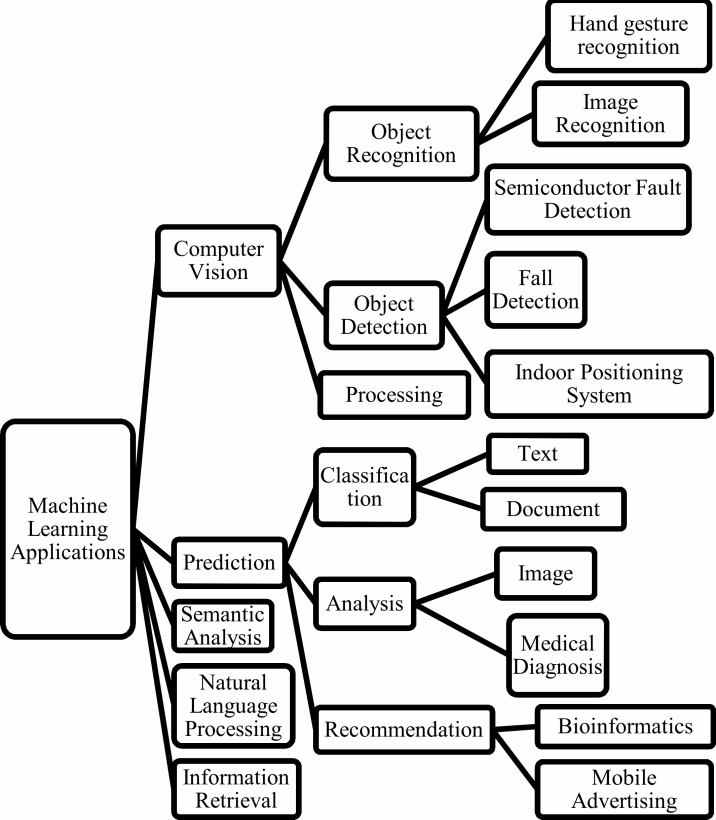
\includegraphics[width=0.7\linewidth]{figuras/mlapplications.png}}
            {Fonte: Extraída de \cite{ApplicationMachineLearning}}
    \label{fig:mlapplications}
\end{figure}

\lipsum[7-8]

\section{Motivação}

Como apresentado em \cite{MLBigdata}, com o resultado do desenvolvimento das tecnologias web, das redes sociais e dispositivos móveis, ocorreu uma verdadeira explosão no crescimento dos dados. 

\lipsum[9-16]


\section{Categorização do problema}

\lipsum[17-18]

\section{Proposta do trabalho}

\lipsum[19-21]

\section{Estrutura dessa trabalho}

O restante deste texto está organizado da seguinte forma. A Seção~\ref{cap:referencial_teorico} apresenta os conceitos básicos do referencial teórico necessário para um melhor entendimento do trabalho, com a apresentação dos assuntos tal, tal e tal. A Seção~\ref{cap:trabalhos_relacionados} contextualiza outros trabalhos que realizaram trabalhos similares. A Seção~\ref{cap:proposta_de_pesquisa} lista as questões da pesquisa, bem como seu objetivo principal e concluindo com as contribuições esperadas com o resultado final do trabalho. A Seção~\ref{cap:metodologia} demonstra qual foi a metodologia do trabalho. A Seção~\ref{cap:experimentos} explica como os experimentos foram executados. A Seção~\ref{cap:resultados} apresenta os resultados dos experimentos, Pot fim a Seção~\ref{cap:conclusao} apresenta um sumário dos resultados e sugestões para trabalhos futuros. 